\documentclass[]{report}
\usepackage[T1]{fontenc}
\usepackage[utf8]{inputenc}
\usepackage[english]{babel}
\usepackage{csquotes}
\usepackage{lmodern}
\usepackage{graphicx}
\usepackage[backend=biber,style=numeric]{biblatex}
\usepackage[hidelinks]{hyperref}
\usepackage{url}
\usepackage{siunitx}
\usepackage{authblk}
\usepackage{subcaption}
\usepackage{tocbibind}
\usepackage{tikz}
\usepackage{amsmath}
\usepackage{pdfpages} %Include pdfs
\usetikzlibrary{calc}

\addbibresource{bibliography.bib}

% text overline command
\makeatletter
\newcommand*{\textoverline}[1]{$\overline{\hbox{#1}}\m@th$}
\makeatother

% Title Page
\title{Ping pong ball catcher}
\date{December 19, 2014}
\author{Anders Jensen\thanks{\url{anje111@student.sdu.dk}}}
\author{Jorge Rodriguez Marin\thanks{\url{jorod14@student.sdu.dk}}}
\author{Kim Lindberg Schwaner\thanks{\url{kschw10@student.sdu.dk}}}
\affil{University of Southern Denmark\\Faculty of Engineering\\EMB1}

\begin{document}

\maketitle
%!TEX root = ../../report.tex
\chapter*{Abstract}
This paper describes the design and implementation of a ping pong ball catcher.
The purpose of the system is to catch a ball, dropped onto a platform, after it has bounced once.
The point of impact of a ball can be determined based on time-difference of arrival of the waves expanding through the platform material from the impact point.
A platform consisting of a square base with four piezoelectric sensors in the corners, and an actuated arm with a net attached, is built.
Analogue circuits are designed to pre-process sensor signals to interface with an FPGA. A component to precisely measure time differences is written in VHDL.
Fast calculation of the impact point in implemented in C on a soft microprocessor.
A desktop GUI application is programmed to obtain and visualise data for each ball hit.
The measurements of time differences turn out to be too inconsistent to always catch the ball.

\tableofcontents
\chapter{Introduction}
\label{chap:introduction}

	\section{Overall description}
		The goal of this project is catching a ping pong ball released above a platform, on which four piezoelectric elements are placed in a rectangular pattern.
		Once the ball has hit the platform once, each of the piezo elements will generate a signal and permit triangulation of the impact point. When the impact point has been found, a net will catch the ball when it returns toward the platform after the first bounce.

		This project has background similar projects as described in \cite{electronic_target} where kind of this system is used for find out the hit's position of a bullet. Also in \cite{tdoa_book} and \cite{tdoa_notes} this method is described and proved. This background motives more the project because it shows that the idea it is possible and reachable.

	\section{Report structure}
	\label{sec:reportStructure}
		The report is structured as follows. To start, the overall design principles \ref{chap:overall_design_principles} where the first theoretical approach to the problem is presented.
		Then, the mechanical view of the project is presented, analysed and solved \ref{chap:mechanics}.
		Follows with the electronics part where the same point of view is done \ref{chap:electronics}.
		Continues with the programming part where two parts are differentiated, the low-level programming and the high-level.
		In the first one \ref{chap:low_level_programming} the VHDL and MicroBlaze sections are treated while in the high-level programming \ref{chap:high_level_programming} the explanation of the computer program is.
		To conclude, the report finish with the experiments carried out \ref{chap:experiments}, the discussion \ref{chap:discussion}, where future lines are commented, and the conclusions \ref{chap:conclusion}.
		At the end can be found appendix as the mechanical drawings \ref{chap:mechanical_drawings}, the Digi diagrams \ref{chap:digi_diagrams} and the equipment used for the project \ref{chap:equipment}.

\chapter{Methodology and Equipment}
\label{chap:methodology}
	In order to complete the project a number of methods and materials were used.

<<<<<<< HEAD
In order to complete the project a number of methods and materials were used.
\section{Methodology}
\label{sec:methodology}
The workload in this project can be divided into PCB-design, manufacturing and high- and low-level programming. Since the workload is large in the low-level programming all multiple people were working on it. Whereas the workload for the other parts were mainly distributed to individuals, to maximize resource utility.   

\subsection{PCB Design and manufacturing}
The design for PCB with the piezo electric elements were conducted by first doing some research on the working principles of the piezo. Since it turn out to be rather hard to theoretically design the PCB  a more pragmatic approach were conducted. 
The sensor characteristics were analyzed by mounting it with a big potentiometer in parallel and measuring the generated voltage when hitting the base plate with a ping pong ball.
Based on this analysis a prototype where put together and tested on a breadboard. 
Then the design from the breadboard are drawn as a schematics and a board in eagle. 
After verifying the schematics and board one of the four identical PCB's are manufactured and tested before producing the others.
Other simpler electrical connections are manufactured on stripboards to minimize time spend on producing PCB's.

\subsection{Low-level programming}
=======
	\section{Methodology}
	\label{sec:methodology}
		The whole project can be divided in four parts that will be treat separately, being this: $mechanics$, $electronics$, $programming$ and $computer program$. At the same time this tasks were organized so:

		In the mechanics part the schedule was:
		\begin{itemize}
			\item Design of the structure
			\item Manufacturing of the laser cutter machine parts
			\item Manufacturing of the 3D printed parts
			\item Structure assembly
			\item Add sensors and electronics to the whole structure
		\end{itemize}

		In turn, the electronics part:
		\begin{itemize}
			\item Circuit design
			\item First prototype test in breadboard
			\item Manufacturing of the PCB boards
			\item Testing
		\end{itemize}
>>>>>>> origin/master

		Whereas in the programming part:
		\begin{itemize}
			\item \textcolor{red}{Blabla}
		\end{itemize}

<<<<<<< HEAD
\subsection{High-level programming}


\subsection{Design and manufacturing of mechanical part}
=======
		To finish, the computer program was divided in:
		\begin{itemize}
			\item UI conceptualization
			\item Serial research and first test
			\item Develop of the whole program
			\item Testing
		\end{itemize}

	\section{Equipment}
	\label{sec:equipment}
		To develop and test the designed solution the following equipments were used.
		\begin{itemize}
			\item Oscilloscope
			\item Multimeter
			\item Soldering iron
			\item \textcolor{red}{FPGA Spartan 3??}
			\item Eagle 7.1 Light
			\item Breadboard
			\item PCB development instruments
			\item Printer
			\item DC servo motor
			\item Murata piezo sensor 7BB-20-6L0
			\item 3D printer
			\item Laser cutter machine
		\end{itemize}
>>>>>>> origin/master

\chapter{Detecting xy-position of ball impact}
This chapter describes the implementation of a solution that enables detection of point of impact for a ping pong ball using an FPGA and piezo electric elements.

\section{TDOA positioning in a plane}
\label{tdoaPositioning}
In this section the relationship between differences in time measurements from multiple sensors and the xy-position of the emitter are derived.
The problem can be modeled as in figure \ref{fig:tdoa_model} where the following parameters are known from the setup and measurements:
\begin{itemize}
	\item Time of arrival of sound at sensors a, b, c and d.
	\item Speed of sound in chosen material.
	\item Position of sensors.
\end{itemize}
The system is setup with four sensors since the possibility of resulting in multiple solutions when using only three \cite{tdoa_book}
The solution will be represented as a system of linear equations to enable fast and relatively simple implementation in VHDL.
The derivation will be conducted for two of the sensors giving one row in the equation system. The other two rows are determined in a similar manner.
\begin{figure}[htb]
	\centering
	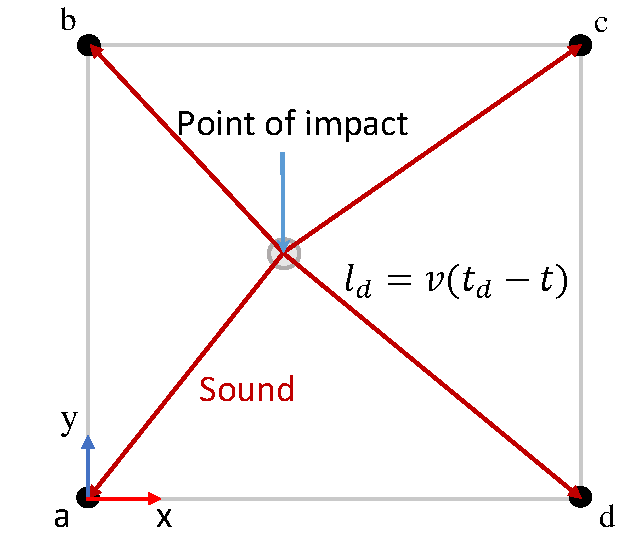
\includegraphics[width=.6\textwidth]{figures/tdoa_model}
	\caption{Side view of the platform surface area and the net. The red markings are piezoelectric sensors.}
	\label{fig:tdoa_model}
\end{figure}

By assuming a constant speed of sound through the impact plane, equation \ref{eq:speedOfSoundDistA} describes the relationship between time difference between measurement and impact $(t_a - t)$ and the distance the impact point is from sensor a.
\begin{equation}
	l_a = v(t_a - t) \Leftrightarrow l_a^2 = v^2(t_a - t)^2 
	\label{eq:speedOfSoundDistA}
\end{equation}
Equation \ref{eq:speedOfSoundDistB} describes the same relationship with respect to sensor b. 
\begin{equation}
	l_b = v(t_b - t) \Leftrightarrow l_b^2 = v^2(t_b - t)^2
\label{eq:speedOfSoundDistB}
\end{equation}
By differencing equation \ref{eq:speedOfSoundDistA} and \ref{eq:speedOfSoundDistB} equation \ref{eq:distanceDiffRelativeToTime} can be derived using the difference of squares formula. It is a linear relation with respect to time of impact $t$.
\begin{equation}
	l_a^2 - l_b^2 = v^2(t_a^2 - t_b^2) - 2 v^2 (t_a - t_b) t
	\label{eq:distanceDiffRelativeToTime}
\end{equation} 
By using Pythagoras theorem the difference in squared distances from the impact point are also related according to equation \ref{eq:distDifference}. It can be seen that it is a linear equation in x and y with constants given from the setup.
\begin{equation}
	\begin{split}
		l_a^2 - l_b^2 & = (x_a - x_b)^2 + (y_a - y)^2 - ((x_b-x)+(-y_b - y))^2 \\
		& = -2( (x_a - x_b) x + (y_a - y_b) y ) + x_a^2 +y_a^2 -(x_b^2 + y_b^2)
	\end{split}
	\label{eq:distDifference}
\end{equation}
By setting equation \ref{eq:distanceDiffRelativeToTime} and \ref{eq:distDifference} equal and isolating the constants known from time measurements and setup equation \ref{eq:firstRow} is derived.
\begin{equation}
	(x_a - x_b) x + (y_a - y_b) y - v^2(t_a - t_b) t = (x_a^2 +y_a^2 -(x_b^2 + y_b^2) - v^2(t_a^2 - t_b^2))/2 \equiv k_{ab}
	\label{eq:firstRow}
\end{equation}
Using similar relations for the other four sensors results in the system of linear equations \ref{eq:linsys} which solution uniquely defines the xy-position of the impact \cite{toa_notes}.
\begin{equation}
	\begin{bmatrix} 
		x_a - x_b & y_a - y_b & - v^2(t_a - t_b) \\
		x_b - x_c & y_b - y_c & - v^2(t_b - t_c) \\
		x_c - x_d & y_c - y_d & - v^2(t_c - t_d) 
	 \end{bmatrix}
	 \left[ \begin{array}{c} x \\ y \\ t \end{array} \right] = \left[ \begin{array}{c} k_{ab} \\ k_{bc} \\ k_{cd}\end{array} \right] 
	 \label{eq:linsys}
\end{equation}
\section{Piezo electric elements}
\label{piezo}
This section describes the construction of a number of sensor circuits using piezo electric elements to measure the time of arrival of bending waves.
There is a circuit like the one on figure \ref{fig:print} for each sensor. It is chosen to make one print for each circuit in order to keep the wires conducting the analog sensor values as small as possible. 
\begin{figure}[htb]
	\centering
	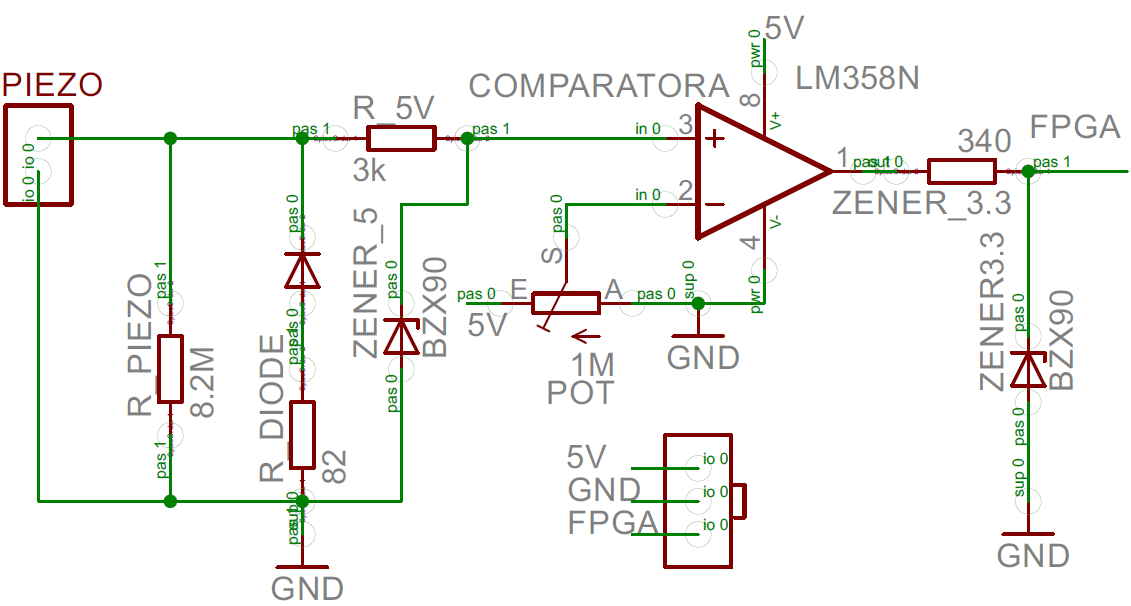
\includegraphics[width=1.\textwidth]{figures/Print}
	\caption{Schematics of circuit for digitalizing the output from a piezo electric elements.}
	\label{fig:print}
\end{figure}
The very small current that the piezo electric element generates are amplified with a resistor on $8.5M\Omega$. This value is chosen since test showed that it was possible to detect ball bounce from as low a hight as $30\si{cm}$.
Diodes are used to account for the large positive and negative voltage spikes that the sensor in combination with the large resistor can output in case of a powerful input to the sensor. 
Since the negative voltage are not use it is removed up to $0.7V$ with a diode which conducts current for ground when the voltage from the piezo becomes less then $0.7V$.
The resistor is calculated according to equation \ref{eq:distDifference}.
\begin{equation}
 20 - 0.7 V = R_{diode} \cdot 300mA \Leftrightarrow R_{diode} = 64.3\Omega 
 \label{diodeResistor}
\end{equation}
Since this resistance was not in stock a resistor of $82 \si{\Omega}$ is chosen.
Where the $20V$ is taken as a guess on the absolute maximum based on the fact that tests has not shown voltages above $15V$ when throwing the ball against the plate. Hence the system are robust against misuse.
Since the op-amp can not compare values that are larger than the supply of $5V$, the positive voltage is limited to $5.1V$ with a zener diode \cite{zener}. The resistor $R_5V$ is calculated by assuming infinite input resistance in the op amp according to equation 
\begin{equation}
20 - 5 V = R_{5V} \cdot 5mA \Leftrightarrow R_{diode} = 3\si{k\Omega} 
\label{eq:zener5VResistor}
\end{equation}
A zener diode \cite{zener} is used to convert the $5V$ on the data output from the operational amplifier to $3.3V$, which is appropriate voltage for the FPGA. The solution with a zener diode is chosen over a another using a voltage divider since the voltage is kept at $3.3V$ for all op-amp of the type LM358 even in case of changes in production. According to the datasheet for LM358 the saturated output voltages varies from the supply voltages down to $1.5V$ below \cite{lm358}.
The resistor placed on the output of the operational amplifier is calculated using the current used for testing conditions in the datasheet for the diode, as can be seen in equation \ref{eq:zener} \cite{zener}.
\begin{equation}
5-3.3V = R_{z} I_{test} \Leftrightarrow R_{z} = 1.7V/5mA = 340\Omega
\label{eq:zener}
\end{equation}
% 
A potentiometer is connected to the inverting pin of the Op-amp in order to ease the tuning process. It's value is set to $1\si{M\Omega}$ to minimize the power consumption.
\section{Construction of impact plane}
\label{impactPlane}

The physical platform area will be a flat area of approximately $40\times40\,\si{\centi\meter}$.
\section{Solving the TDOA using VHDL}
\label{TDOAVHDL}
This section describes how the solution for TDOA positioning are implemented in VHDL on a FPGA.

\subsection{Precise timing}

\subsection{Solving system of linear equations}

\section{Microblaze MCS}
A Microblace micro controller system(MCS) is used for handling the following tasks in descending priority:
\begin{itemize}
	\item Fast and precise solution to the TDOA problem.
	\item Calculating inverse kinematics for the robot arm.
	\item Handling UART communication with a PC.
\end{itemize}
The choice of using a MCS is due to expediency in the implementation.

\subsection{Setup of Microblaze IP-core} 
It is chosen to implement the solution of the TDOA problem in Microblaze MCS version 1.4. This soft core microcontroller implemented on an FPGA is used rather than developing the solution directly in VHDL. 
The reason for this choice is that it is easier to implement the commonly used numerical methods for solving systems of linear equations in a sequential order rather than in parallel. 
The smaller and older Picroblaze MCS is avoided since xilinx does not support a C compiler  
($http://forums.xilinx.com/t5/PicoBlaze/PicoBlaze-FAQ-Is-there-a-C-Compiler/td-p/580$). 
The Microblaze system with more than 4k of memory has proven take up more than the 50K logic gates available on the XC3S50AN, that is mounted on the previously use development board ($http://www.xilinx.com/support/documentation/data_sheets/ds557.pdf$). 
This small memory size is too small for easy implementations which often includes large programs. As an example of a nice function that takes op a lot of program space is the printf function, that is very useful for debugging.
Due to these limitations the more suitable Nexus 2 board is used which includes an Spartan-3E with 500K gates.  

The Microblace MCS is included in the VHDL project as an IP-core using the IP-core generator GUI in ISE-design suit. Here the settings are left at their default values unless otherwise needed. The memory size is assigned to 32k since test showed sufficient space on the FPGA for this. The UART is setup to transmit and recive at a baud rate on 115200 without using interrupts. Four general purpose inputs(GPI) with a size of 32 bits is used to receive four timings values. The 32 bits precision is used since the Microblaze has a is a 32-bits processor. Two general purpose outputs(GPO) is used. One of them contains the newest calculated angle from the inverse kinematics and the other one is used as a flag indicating that a new angle is available. One external interrupt is used to initialize the calculation of the TDOA problem. 

\subsection{C-program on Microblaze}
The program running on the Microblaze is built op rather simple with a setup followed by a while true loop responding with results of the TDOA problem upon request from the PC-program. Since there is rather strict timing constrains on calculating the inverse kinematics in order to move the arm under the ball before a second hit the calculations are handled in a interrupt service routine. The program is build using standard math utilities and specialized Microblace tools for GPIO, interrupts and UART.

\subsection{Interrupts on Microblaze}


\subsection{Solve TDOA}
The solution to the TDOA problem is handled by solving the system of linear equations described in section TODO:(intro about TDOA reference). To keep implementation simple the solution is implemented with gauss elimination. Software implemented floating point precision are used in the calculations due to the fact that the used free version of Microblaze does not include a floating point arithmetic unit. 
The gauss elimination is implemented by running through each column and for each do the following (Source Numerical analysis):
\begin{itemize}
	\item Pivoting by sorting the from top to bottom rows according to descending pivot elements.
	\item Eliminate elements in column under current pivot element by subtracting the current row multiplied with the element in the pivot column under the pivot element under consideration divided with the pivot element.
\end{itemize}

When the iterations reaches the last column the coefficient matrix is on an upper triangular matrix form. This enables back substitution starting from the button row and calculating the solution x based on the previous calculated solution as can be seen in equation.
\begin{equation}
	x_n = \frac{b_n}{a_{nn}}
\end{equation}

\begin{equation}
	x_i = \frac{1}{a_{ii}} (b_i - \sum_{j=i+1}^{n-1} a_{ij}x_j)
\end{equation}
Where a is the coefficient matrix, b is the right hand side vector and n is the number of rows and columns.

The inverse kinematics are calculated using $atan(y/x)$ where $y$ and $x$ are the calculated coordinates of the impact point. 

\subsection{GPIO and UART}

% \chapter{Height of ball bounce back}
\label{bounceBack}

\section{Determerning energy in impact using ADC}

\section{Bounce back height from measured energy}
Derive the kinematics for the ball bouncing back.
\chapter{Two joint arm as ball catcher}
\label{catcherArm}
	A arm will be mounted on a stick besides the platform so that the net does not hit the ground. The arm consist of two

	\section{Physical construction}
	\label{armConstruction}
		How the arm is constructed to be robust and fast while being able to reach the specified area for impact.


	\section{Inverse kinematics and control}
	\label{kinematics}
		Due to the construction of this prototype with just one servo, the position of the servo is defined by:

		$$\theta = \arctan\frac{y}{x}$$


\chapter{PC Program}
\label{chap:pc_program}
	A PC program shows the position of the hit and save a history where the user can see all the hits in the session along with the position.

	\section{Communication and Logic}
	\label{sec:pc_program_com}
		Regarding the communication, the PC program and the FPGA are connected by a USB wire and this protocol is handle by the Qt serial libraries given. 
		This let the communication in hands of a code that has been already tested. 
		The use of Qt let the user compile and use this program in any operative system which gives to the user freedom to use the machine in more conditions.

		The program is the master in the communication, and it try to establish communication by default from the beginning. 
		While there are a default connection options, a settings window has been implemented so the user can change the options easily. 
		This options are: $Baud Rate, Parity, Stop Bits, Flow Control$ and $Local Echo$.

		Once the communication is establish, the program send a character that the FPGA interprets as $send hit information$. 
		Then, the FPGA sends through the USB the $x$ and $y$ coordinated along with a $hash$ of the hit, that defines a unique identifier for it. 
		If the hit is a new hit, the program shows it in the UI and save it in the history so the user can see them again when desired.

	\section{Interface}
	\label{sec:pc_program_interface}
		The UI has been developed so the user can easily configure the connection and see the hits. 
		On one hand, the connection is establish automatically from the start, so the user has not to do anything. Furthermore the hits, are immediately shown in a intuitive square that represents the platform where the sensors are allocated.

		On the other hand, the interface only has two buttons. The first one is $Settings$ and it opens a window where the connections parameters can be configured. The second is $History$ and, when clicked once, it shows all the hits positions in that session. If clicked again, the program come back to detect more hits.

		Summering up, the program let have a pretty and easy to use interface between the machine and the user giving the opportunity to all kind of users being able to use it. Furthermore it stores a graphical history for further researches.

		\begin{figure}[hb!]
			\begin{center}
				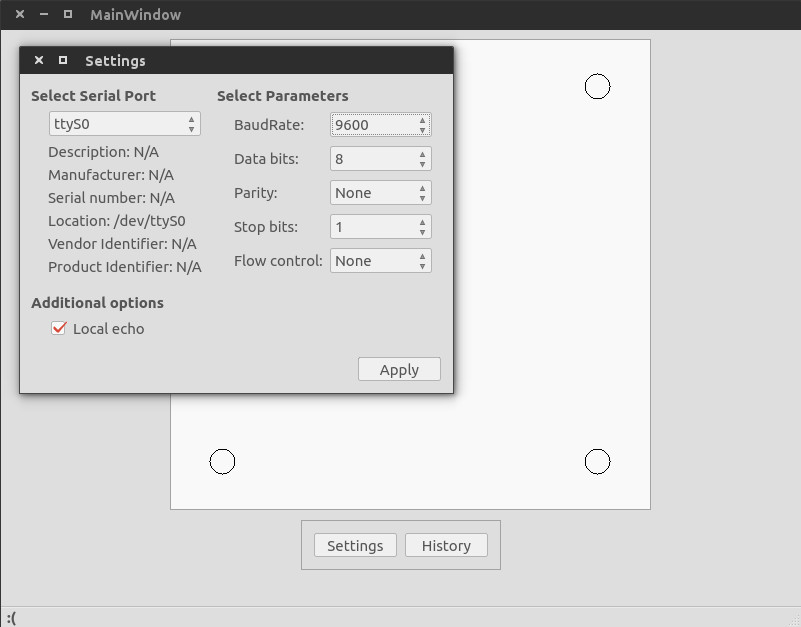
\includegraphics[width=.8\textwidth]{figures/UI}
			\end{center}
			\caption{UI of the program}
			\label{fig:ui}
		\end{figure}
\chapter{Conclusions}
\label{chap:conclusions}

	After the design, implementation of the project and have carried out all the experiments to determine the reach of the machine we are able to conclude that:
	\begin{itemize}
		\item Despite the 
	\end{itemize}

\nocite{*} %To print the no referencered referencies
\printbibliography[heading=bibintoc]

\appendix
\chapter{Mechanical drawings}
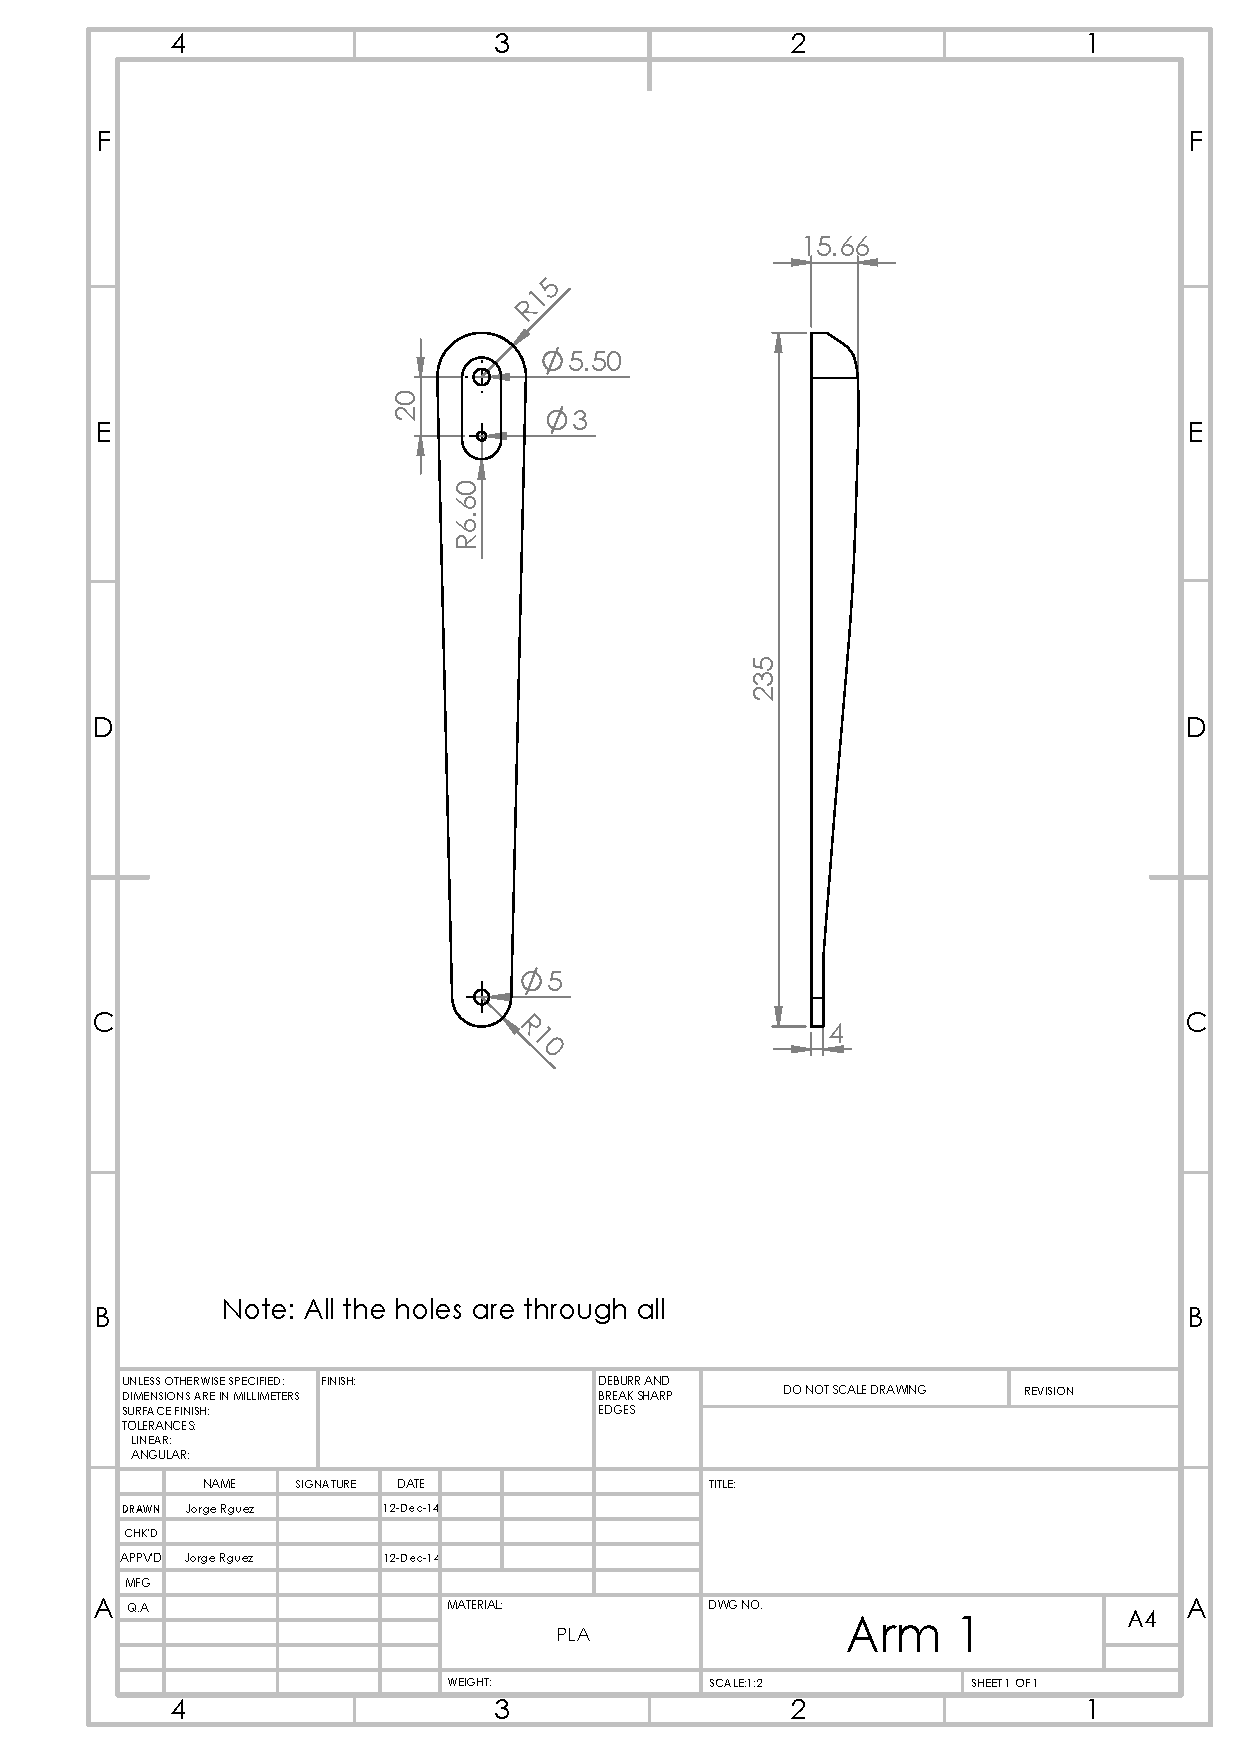
\includepdf[pages={1-7}]{includes/planes.pdf}

\chapter{Digital circuit design diagrams}\label{cha:digi-diagrams}
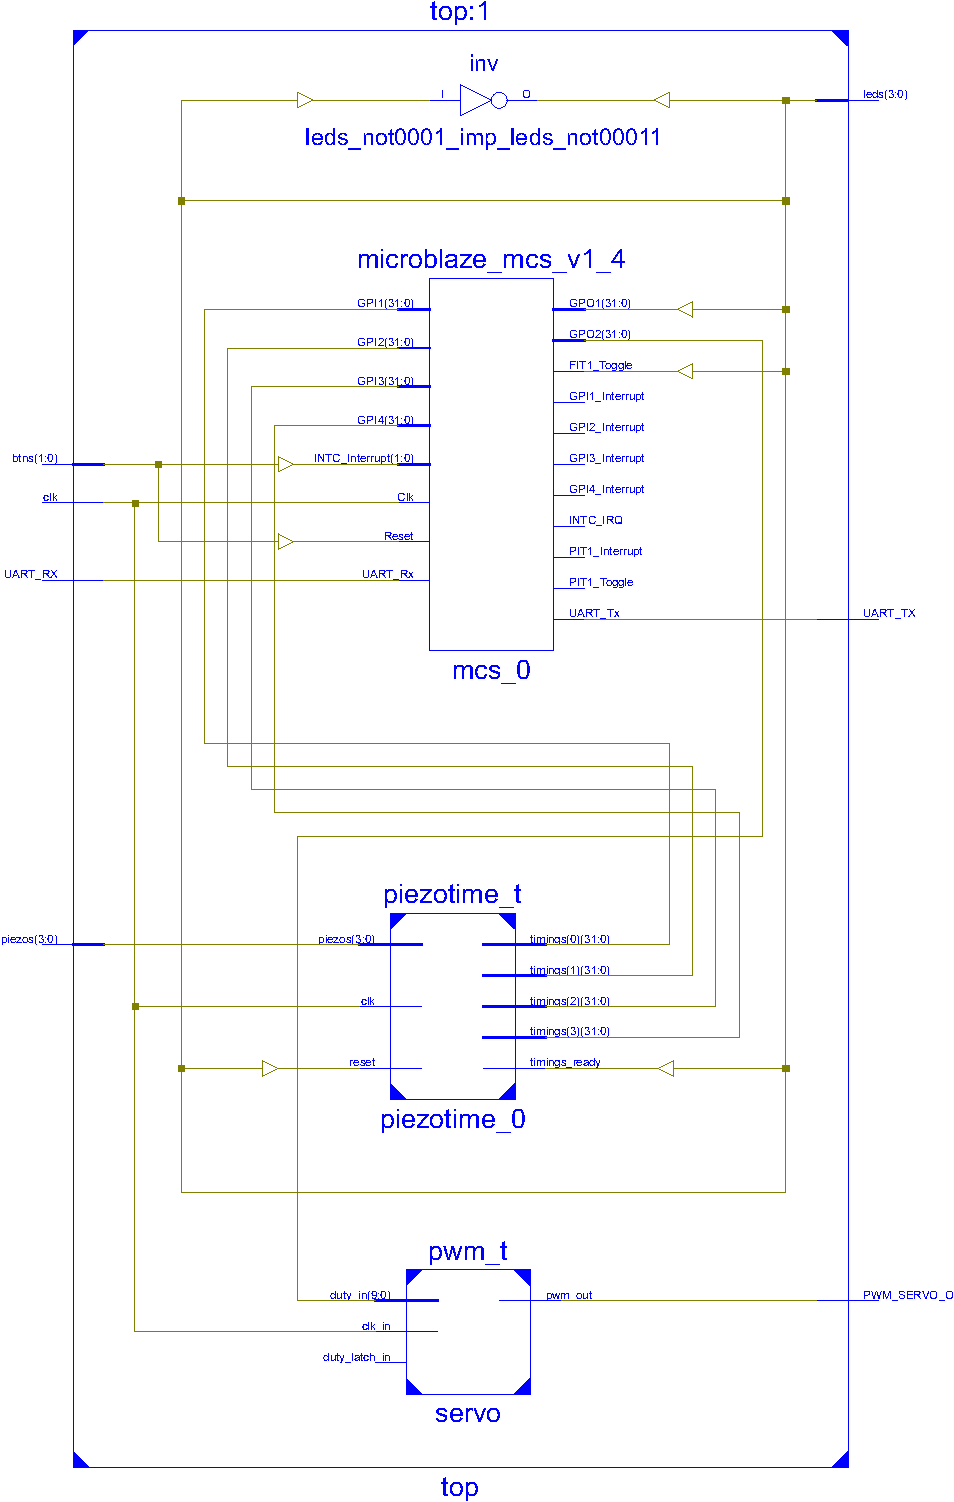
\includepdf[]{figures/rtl-sch.pdf}
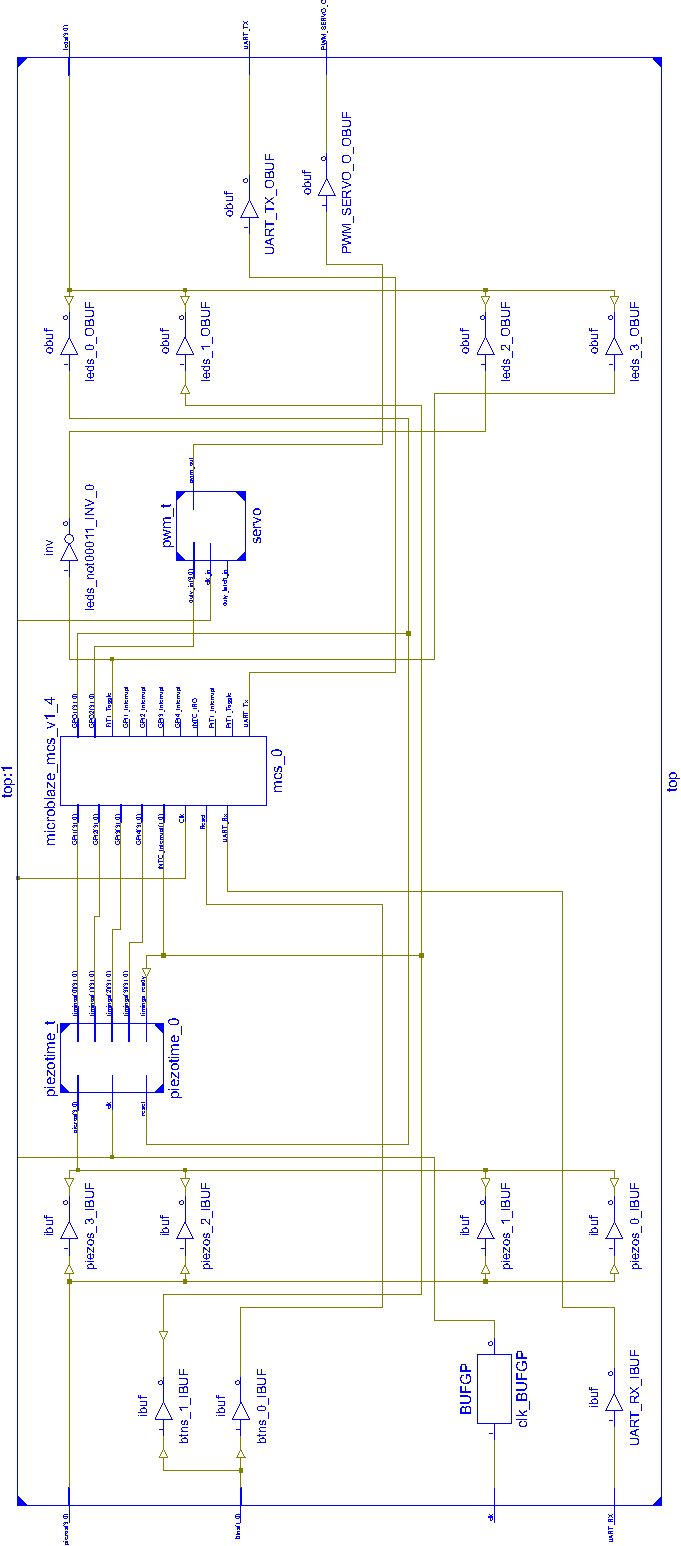
\includepdf[landscape]{figures/tech-sch.pdf}

\end{document}
